% Chapter Template

\chapter{Code} % Main chapter title

\label{Code} % Change X to a consecutive number; for referencing this chapter elsewhere, use \ref{ChapterX}

\lhead{Chapter 3. \emph{Code}} % Change X to a consecutive number; this is for the header on each page - perhaps a shortened title

%----------------------------------------------------------------------------------------
%	SECTION 1
%----------------------------------------------------------------------------------------

\section{Libraries}
The implementation relies heavily on the \texttt{Eigen}\cite{eigenweb} template library for linear algebra. I have introduced a handful of template aliases to simplify the typenames of the most commonly used objects. Additionally, the code utilizes \texttt{eigen3-hdf5}\cite{eigen3-hdf5} for the serialization of the \texttt{Eigen} matrices into \texttt{hdf5} files.

\section{Matrix Potential}
In this section, I list all of the modules that can be used to create a matrix potential and elaborate on how to combine them.

\subsection{Abstract and Standard Implementation}
Most modules contain a class called \texttt{Abstract} which defines the functionality the module offers and implements some common functionality. This is usually the extension of an evaluation from a single point to a grid of points. Each module then provides at least one implementation (if only one implementation is provided, it is called \texttt{Standard}) of \texttt{Abstract} which inherits from \texttt{Abstract} using static polymorphism as described in the previous chapter. To add his or her own implementations the user can simply follow the pattern of the standard implementation. As an example, a user could define his or her own implementation of the \texttt{taylor} module wherein all of the evaluations are hard-coded instead of delegated to lambda functions for a more efficient evaluation.

\subsection{Namespaces}
To keep the global namespace and the \texttt{waveblocks} namespace unpolluted with implementation details all matrix potential related implementations are put within their own namespace \texttt{matrixPotentials} which contains a namespace \texttt{modules} which in turn contains a namespace for each module. Only standard implementations are exported via template aliases.

\subsubsection{Bases}
The \texttt{bases} namespace contains the class templates for the basis classes \texttt{Canonical} and \texttt{Eigen}. These are merely a collection of constants and aliases to make templating easier. Instead of a module depending on a large number of types it simply depends on a \textit{basis} and imports the required types via a macro.
\texttt{Canonical} and \texttt{Eigen} are exported to the \texttt{waveblocks} namespace via template aliases.

\subsubsection{Potentials}
The \texttt{potentials} namespace contains template aliases for often used configurations of modules such as a scalar valued potential which supports evaluation of the local quadratic remainder.

\subsubsection{Modules}
\begin{itemize}
\item \texttt{evaluation}: allows to evaluate a potential in one or many points
\item \texttt{jacobian}: allows to evaluate the Jacobian as defined in Chapter \ref{Introduction} in one or many points
\item \texttt{hessian}: allows to evaluate the Hessian as defined in Chapter \ref{Introduction} in one or many points
\item \texttt{exponential}: allows to evaluate the exponential of the resulting matrix of an evaluation in one or many points
\item \texttt{taylor}: allows to evaluate the potential, Jacobian and Hessian all at once in one or many points
\item \texttt{localQuadratic}: allows to evaluate the local quadratic of a matrix potential as defined in Chapter \ref{Introduction}
\item \texttt{leadingLevelOwner}: allows to define a potential which owns another potential
\item \texttt{localRemainder}: allows to define a potential whose local quadratic remainder can be computed as defined in Chapter \ref{Introduction}
\end{itemize}

\paragraph{Standard Implementations}
Figure \ref{fig:dia} shows the class diagram of the standard implementations of the modules available. Note that this class diagram only holds when using the template aliases provided by each module (i.e. using \texttt{waveblocks::Evaluation} rather than \texttt{waveblocks::matrixPotentials::modules::evaluation::Standard} as the standard implementations are usually more general and allow passing the super class as a template argument in most cases.
\begin{figure}
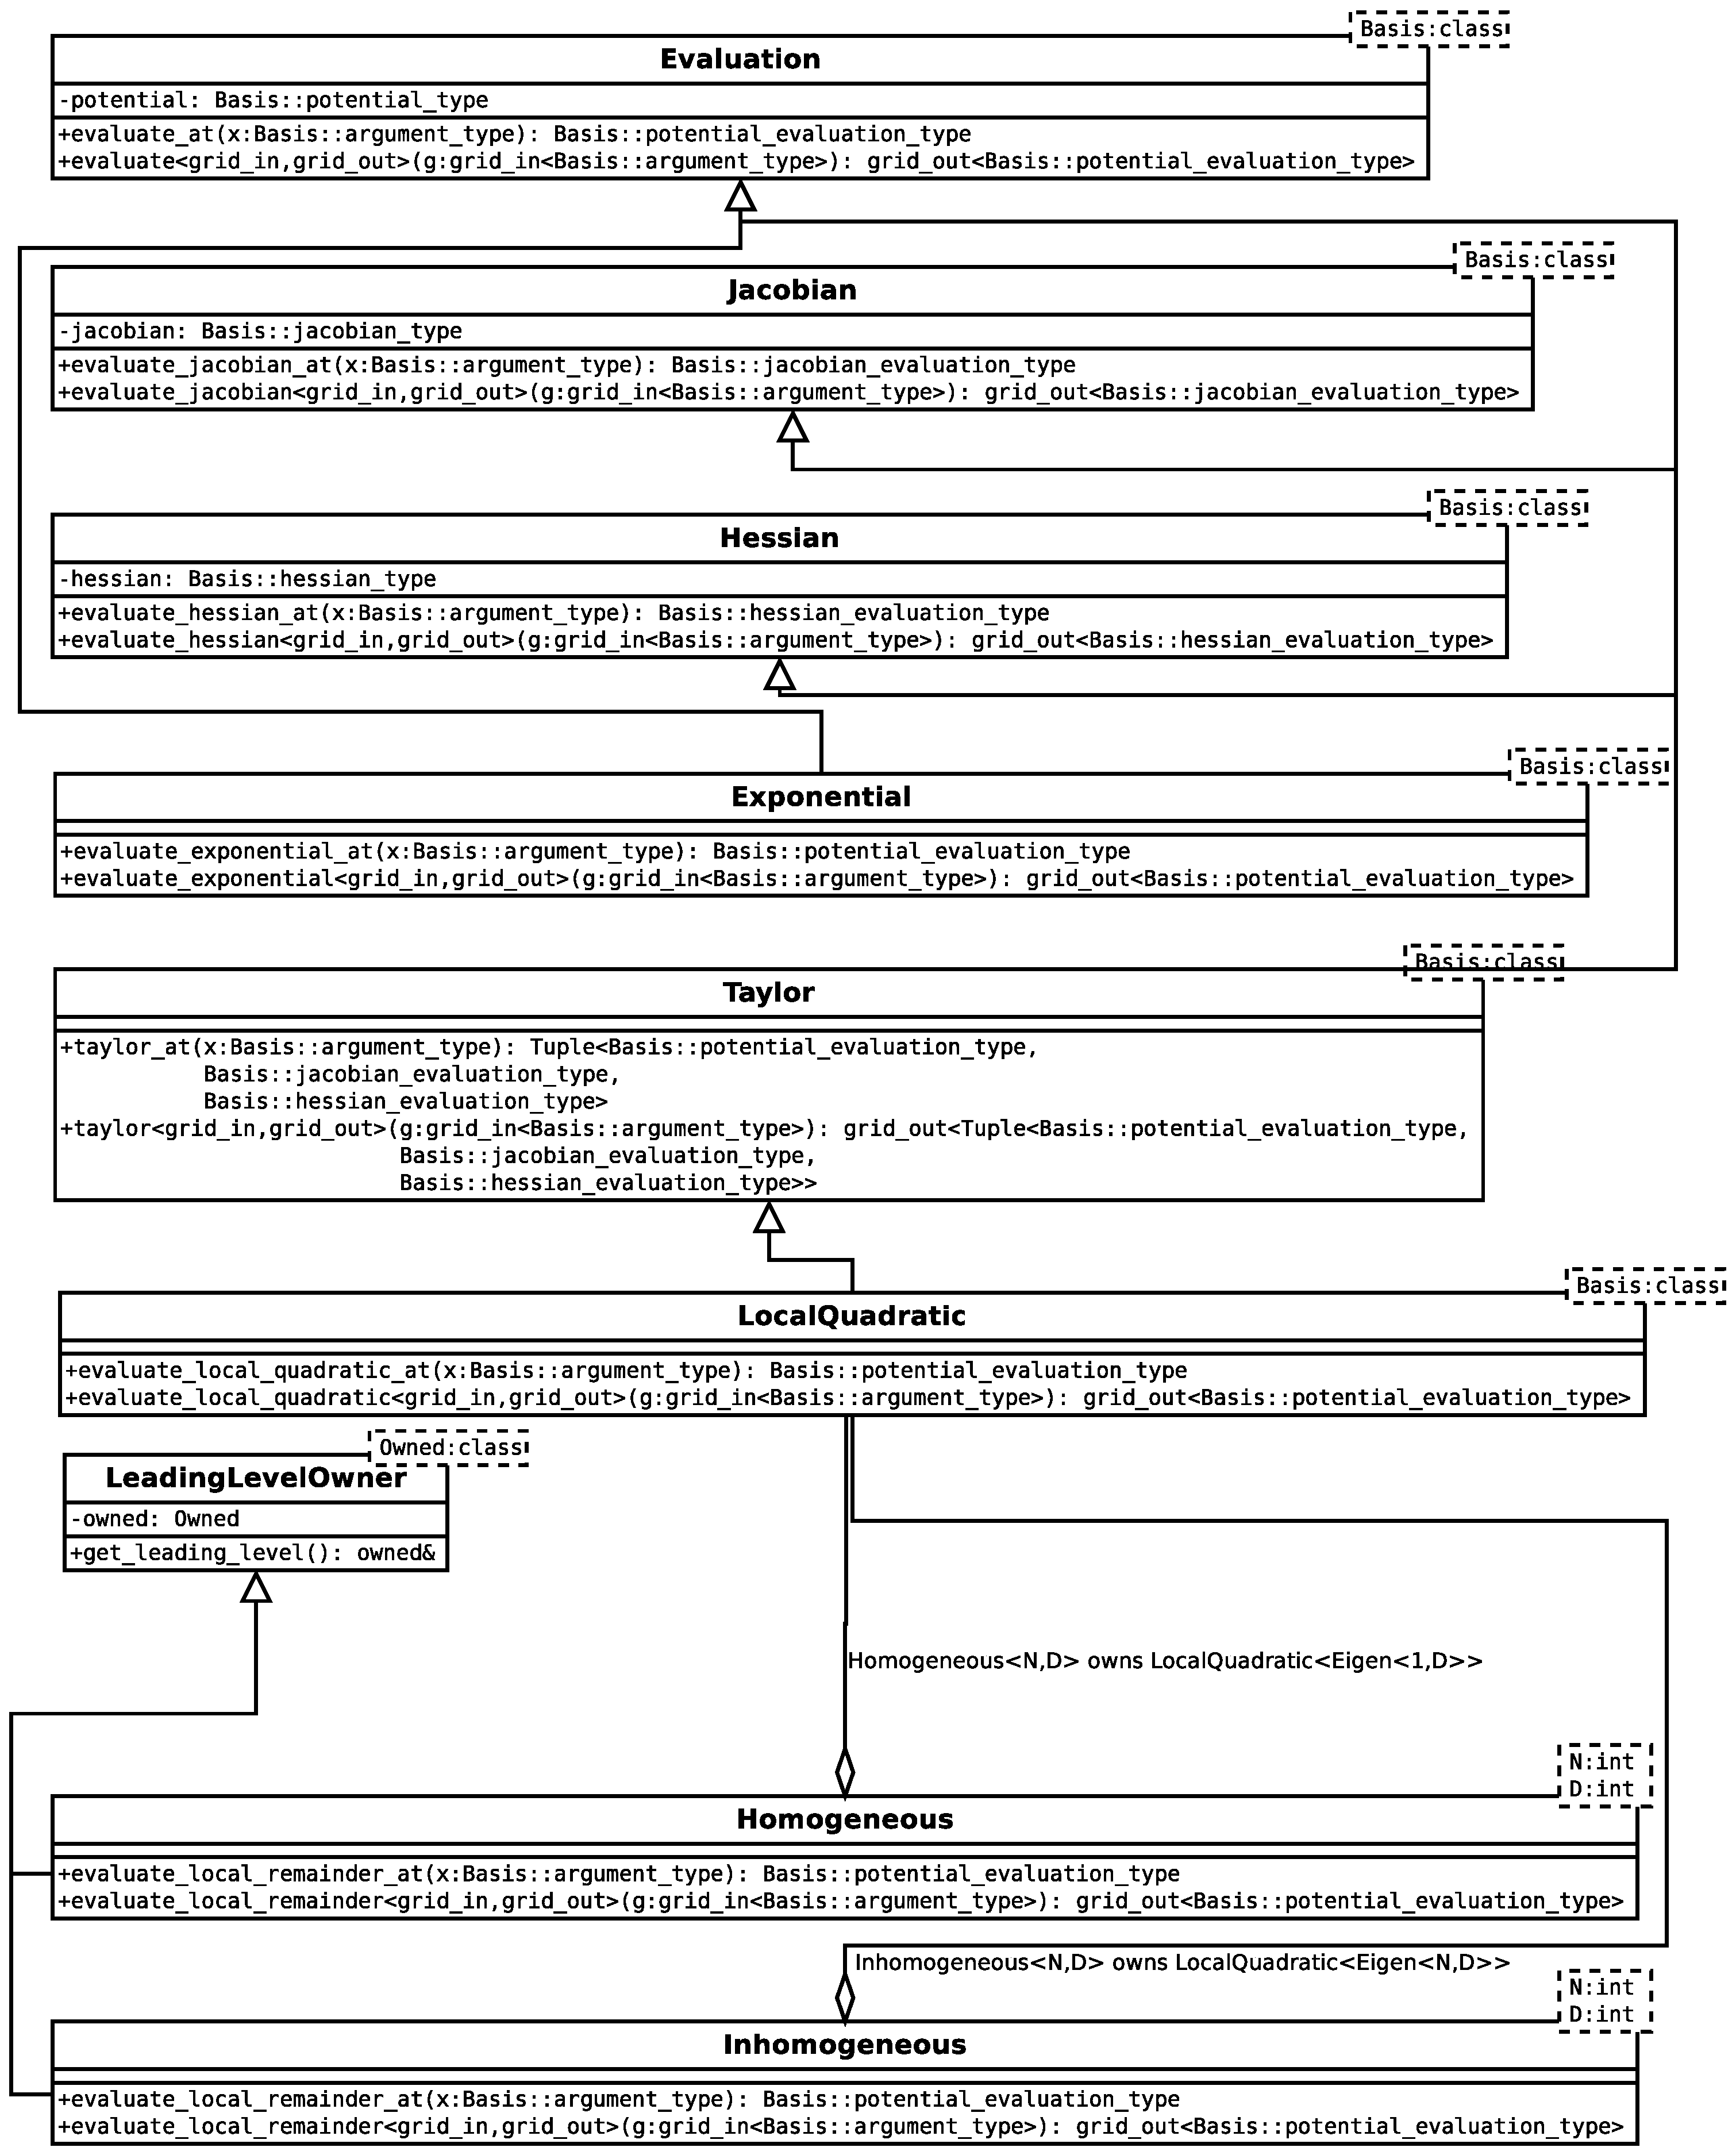
\includegraphics[width=\textwidth]{Figures/standardModules.eps}
\caption{Diagram of the standard implementations of the modules available and their class hierarchy. All of these classes are available in the \texttt{waveblocks} namespace.}
\label{fig:dia}
\end{figure}
\section{Hagedorn Propagator}
The Hagedorn propagator is implemented as a template class templated on the number of levels $N$, the dimension $D$, as well as the class \texttt{MultiIndex}, used for indexing the wavepacket, and the class \texttt{TQR}, which defines the tensor quadrature rule.
It offers the static method propagate which is overloaded for homogeneous and inhomogeneous wavepackets and specialized for scalar wavepackets. 
The propagator needs different implementations for $N=1$, $N>1$, $D=1$, $D>1$ as well as different implementations for homogeneous and inhomogeneous wavepackets. However, there exists a lot of overlap in these implementations which I make heavy use of by delegating non-overlapping parts to partially specialized template functions. As an example we can see that for the first step the inhomogeneous case simply iterates over all components and applies the same operation to the parameter set of the Hagedorn wavepacket propagated as the homogeneous case does. Similarly, there are only a few lines of code that need to be adjusted when dealing with $D=1$.

